\section{Networking in IoT}
\label{sec:domain-survey}
\subsection{The Protocol stack in ICN}

\label{subsec: The Protocol stack in ICN}
It is after years of networking research and development that we are able to use the TCP/IP stack as the default standard for all networking protocols in this age of information. The TCP/IP stack is designed based on the standard OSI Model of different layers, each with different functionalities that in turn help the functionalities of the upper layers. This is basically a complex system of network protocols directly influenced by the lower abstractions up till the application layer that help connect to different users or applications throughout the world. However from the early days, security was not incorporated in the design of this stack. Therefore the foundation of this IP stack always had room for improvement in the security aspect. But such an improvement costs additional overhead to the system that causes lower performance and further delay. At the rate at which technology is advancing computing power has become cheaper but with the advent of IoT devices and the scale at which it has encroached our day to day life requires a second look at the way we use this network stack.\par
In doing so, it was noted that our current applications do not access devices based on who is using it (as it used to in earlier office rooms.) but instead due to globalization, the applications are more content oriented, a user is more likely to find a certain piece of information or content on the Internet rather than from whom it comes. This observation led to the fact that when a user tries to access such an information on the Internet, the network layer goes through several mapped translations before it can send the user this information. This is computationally more work than what it would have been if this data was asked directly. This is where the ICN paradigm comes to play.\par
The ICNs network design is application driven. The current applications such as facebook, spotify , netflix et cetera provide users with some sort of content over the Internet. This content is bound to some sort of identifier which is accessed through the Internet. But is this really efficient? The answer is no. This static information can be referenced in a simpler manner with names rather than creating identifiers over the networks for routing tables to forward around. Thus ICN allows the network layer to have an abstraction that accesses named content rather than addressable end-hosts. In doing so, it also adds the requires security measures to it.\par
It is however crucial to have a separate naming abstraction to provide for globally unique and content relevant naming abstraction above the ICN networking layer. These names not only help to find the location of the device faster but also states which services is this device allowed to access according to the access mechanisms. 

 \begin{figure}[h]
	\centering
	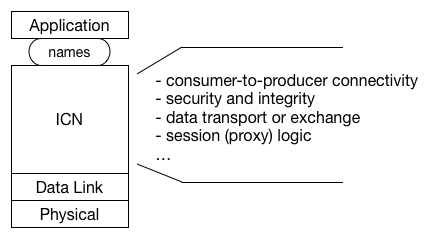
\includegraphics[width=0.8\linewidth]{Figures/stack.png}
	\caption[]{ICN stack}
	\label{fig:stack}
\end{figure}
Here is the traditional stack and its features in Fig. \ref{fig:TCP/IP stack}. 
The IP stacks layers have a network layer (Layer 3), upon that there is the transport layer (Layer 4) that provides end-to-end communication and on top of this there is another layer that proves a secure channel for communication.  As these layers grew to add more functionality, the applications required more APIs to handle the host-centric Internet. Since most of the communication occurred with a simple HTTP get request, all the layers underneath became depended on each other and became almost static in nature. But the idea was always to fetch a particular data and not to reach a particular device. Hence ICN is an ambitious goal to redevelop the layers between the data link and application layer in such a way which is best suited for today's applications that are content driven.\par
In Fig. \ref{fig:stack}, we can see how these layers are merged into a single ICN layer that has a name abstraction before the application layer. The functionalities that are provided are thus, consumer to producer connectivity, security with integrity, data transport and a session logic. This eradicates the technical debt of the network layer of the IP stack.

\subsection{IoT Architectural Requirements}
\label{subsec: IoT Architectural Requirements}
First, we will look at what an IoT systems architectural requirements are. They are as follows:

\subsubsection{Naming}
The names assigned to each device must be globally unique. In an IoT environment where the devices are mobile or migrate from one place to another and have a questionable lifetime.
It is important that the names remain persistent. Therefore more stress on what the device holds as content rather than its locations. Another aspect of naming is that they must be self certifying. That is the names assigned to a particular device must be bound to that particular device and this must be true at all times. This certification must be made by the device itself. 
In ICN, users may either generate their own public keys and submit them to the Name certifying service(NCS) for registration, or may contact the NCS to acquire public keys. This is based on a trust model that the NCS will certify the binding of the name and device and thus provide integrity.
\subsubsection{ Security and Privacy
} The security challenges are data integrity, authentication of users, access control assigned to devices or devices, privacy of data producers and consumers, privacy of the data content or service responses, privacy of contextual information such as time and location of data transmission. These must be included in the system without interfering with the flexibility and usability of the application by users.
\subsubsection{Scalability
}Cisco predicts there will be around 50 Billion IoT devices such as sensors, RFID tags, and actuators, on the Internet by 2020.  As mentioned above, a unified IoT platform needs to name every entity such as data, device, service etc. Scalability has to be addressed at multiple levels of the IoT architecture including naming, security, name resolution, routing and forwarding level. Mobility adds further challenge in terms of scalability. Particularly with respect to name resolution the system should be able to register, update or resolve a name within a short latency. 
\subsubsection{Resource Constraints
} End to end latency is affected by the device constraints such as power, storage, computing constraints. Since the IoT devices are usually low end devices, their constraints must be considered before applications can be successfully be run on them. This especially plays a role in real time applications.
\subsubsection{Traffic Characteristics
}Another form of constraint is traffic constraint. This is due to the presence of neighboring devices that require data filtering or due to wide area update where a broad knowledge base is accumulated. As a result, the traffic characteristics of the IoT services have to be properly accounted for during provisioning the system. 
\subsubsection{Contextual Communication
}Many IoT applications rely on dynamic contexts in the IoT system to initiate, maintain and terminate communication among IoT devices. Here, we refer to a context as attributes applicable to a group of devices that share some common features, such as their owners may have a certain social relationship or belong to the same administrative group, or the devices may be present in the same location. These temporary groups are referred to as contexts. IoT applications need to support interactions among the members of a context, as well as interactions across contexts. 
\subsubsection{Handling Mobility
}There are several degrees of mobility in different IoT scenarios, ranging from static as in fixed assets to highly dynamic in vehicle- to-vehicle environments. Mobility in the IoT architecture can mean either the data producer mobility (i.e., location change), the data consumer mobility, IoT Network mobility (e.g., a body-area network in motion as a person is walking); and disconnection between the data source and destination pair (e.g., due to unreliable wireless links). The requirement on mobility support is to be able to deliver IoT data below an application's acceptable delay constraint in all of the above cases, and if necessary to negotiate different connectivity or security constraints specific to each mobile context. 

\subsubsection{ Storage and Caching
}Storage and caching plays a very significant role depending on the type of IoT ecosystem, also a function subjected to privacy and security guidelines. Caching is usually done for increasing data availability in the network and reliability purposes, especially in wireless scenarios in the network access and with intermittent connectivity to the infrastructure network. Storage is more important for IoT, storing data for long term analysis. \par
Data is stored in strategic locations in the network to reduce control and computation overhead. Furthermore considering hierarchical nature of IoT systems, ICN architectures enable flexible heterogeneous and potentially fault-tolerant approach to storage and caching providing contextual persistence at multiple levels. 
\subsubsection{Communication Reliability
}Reliable communication desires the following capabilities for the underlying system:  seamless mobility support under normal operating conditions,  efficient routing in the presence of intermittent disconnection,  QoS aware routing,  support for redundancy at all levels of a system (device, service, network, storage etc.), and support for rich and diverse communication patterns, both within an IoT domain consisting of multiple IoT nodes and one or more gateway nodes to the Internet and across multiple such domains. 
\subsubsection{Self-Organization
} Self organization is the capability to quickly discover heterogeneous and relevant (local or global) devices/data/services based on the context. This discovery can be achieved through an efficient publish-subscribe service, or through private community grouping/clustering based upon trust and other security requirements. 
\subsubsection{Ad hoc and Infrastructure Mode
}The unified IoT architecture needs to design a common protocol that serves both modes. Such a protocol should address the challenges that arise in these two modes: (1) scalability and low latency for the infrastructure mode and (2) efficient neighbor discovery and ad-hoc communication for the ad-hoc mode.  
\subsubsection{IoT Platform Management
}An IoT platforms' service, control and data plane will be governed by its own management infrastructure which includes distributed and centralized middle-ware, discovery, naming, self-configuring, analytic functions, and information dissemination


\subsection{IoT Middleware architecture}
\label{subsec: IoT Middleware architecture}
 \begin{figure}[ht]
	\centering
	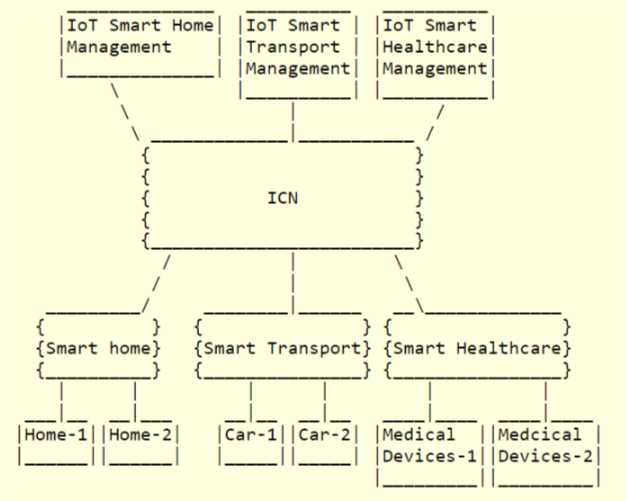
\includegraphics[width=0.8\linewidth]{Figures/archi.png}
	\caption[]{ICN-IoT unified architecture}
	\label{fig:archi}
\end{figure}
\subsubsection{Advantages of using ICN for IoT}
Now that we have seen that all the requirements of an IoT architecture lets see how the ICN architecture fits most of its criteria flawlessly. A key concept of ICN is the ability to name data independently from the current location at which it is stored, which simplifies caching and enables decoupling of sender and receiver. \par
The heterogeneity of both network equipment deployed and services offered by IoT networks leads to a large variety of data, services and devices.  All these can be named exclusively by the ICN layer that can be communicate with each other through these names. These names thus lead to self configuration of devices into groups that simplify caching in strategic points of the network.\par
ICN advocates the model of object security to secure data in the network. This concept is based on the idea of securing information objects unlike session-based security mechanisms which secure the communication channel between a pair of nodes. ICN provides data integrity through Name-Data Integrity.\par
IoT networks can potentially benefit even more from caching and in-network processing systems, because of their resource constraints. Wireless bandwidth and power supply can be limited for multiple devices sharing a communication channel, and for small mobile devices powered by batteries. In this case, avoiding unnecessary transmissions with IoT devices to retrieve and distribute IoT data to multiple places is important, hence processing and storing such content in the network can save wireless bandwidth and battery power. Moreover, as for other types of networks, applications for IoT networks requiring shorter delays can benefit from local caches and services to reduce delays between content request and delivery. \par
 IoT devices may be mobile and face intermittent network connectivity. When specific data is requested, such data can often be delivered by ICN without any consistent direct connectivity between devices. Apart from using structured caching systems as described previously, information can also be spread by forwarding data opportunistically, this allows for sender and receiver decoupling.
\subsubsection{Unified IoT architecture}
Now that we have looked at why ICN can be used for IoT infrastructure, we shall understand about the Middleware that will be considered for the implementation of such an infrastructure to work.
The Middleware is intended to address the administrative services of this architecture such as device/service discovery, user registration and naming. The content delivery is handled by the ICN network. Thus delivering IoT services over the ICN Network.
The proposed ICN-IoT unified architecture is shown in Fig.\ref{fig:archi}.
\par

The five components of the ICN-IoT architecture: are:
\begin{enumerate}
\item Embedded system
\item Aggregator
\item Local Service Gateway(LSG)
\item ICN-IoT Server
\item Service/Consumer
\end{enumerate}
\begin{figure}[ht]
	\centering
	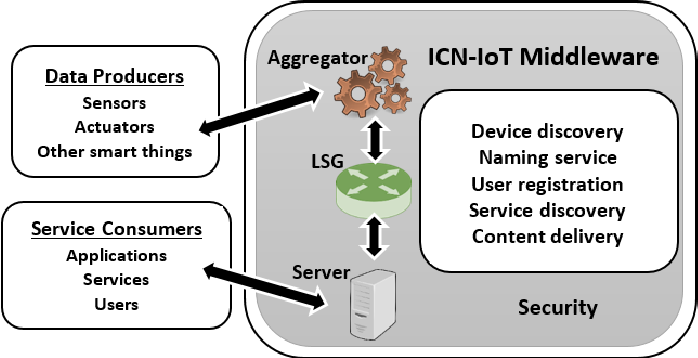
\includegraphics[width=0.8\linewidth]{Figures/Architecture.png}
	\caption[]{Middleware architecture}
	\label{fig:architecture}
\end{figure}
This Fig. \ref{fig:architecture} shows the ICN-IoT Middleware.

Embedded Systems (ES): The embedded sensor has sensing and actuating functions and may also be able to relay data for other sensors to the Aggregator, through wireless or wired links.\par
Aggregator: It interconnects various entities in a local IoT network. Aggregators serve the following functionalities: device discovery, service discovery, and name assignment. Aggregators can communication with each other directly or through the local service gateway.\par
Local Service Gateway (LSG): A LSG serves the following functionalities: (1) it is at the administrative boundary, such as, the home or an enterprise, connecting the local IoT system to the rest of the global IoT system, (2) it serves to assign ICN names to local sensors, (3) it enforces data access policies for local IoT devices, and (4) it runs context processing services to generate information specified by application-specific contexts (instead of raw data) to the IoT server.\par
ICN-IoT Server: Within a given IoT service context, the IoT server is a centralized server that maintains subscription memberships and provides the lookup service for subscribers. Unlike legacy IoT servers that are involved in the data path from publishers to subscribers raising the concern of its interfaces being a bottleneck the IoT server in our architecture is only involved in the control path where publishers and subscribers exchange their names, certificates, and impose other security functions such as access control.\par
Services/Consumer: These are other application instances interacting with the IoT server to fetch or be notified of anything of interest within the scope of the IoT service.\par

\subsection{ICN-IoT Middleware Functions}
\subsubsection{Onboarding}
The objective of onboarding is to connect new devices to the rest and enable them to operate in the ecosystem. Every entity should be exposed to its direct upstream neighbor and may be another embedded system or aggregator. Specifically, it includes the following three aspects: a newly added ES should be exposed to its neighbor (ES or aggregator) and possibly to its LSG, AM, and the IoT server; a newly added aggregator is exposed to its LSG, and possibly to its neighbor aggregators; a newly added AM should be exposed to the IoT server and the LSG; and a newly added LSG should be exposed to the IoT server. Device discovery serves two functions:  it is used in the context of discovering neighboring ESs to form routing paths, where existing mechanims can be used for device onboarding. This has been discussed in later section thoroughly.
\par
In most IoT systems, devices interact with the aggregator for data or information processing or aggregation, hence there is no direct communication between devices under an aggregator. If in some set-up devices under the aggregator need to communicate with each other a scalable mechanism is to allow direct neighbors to communicate with each other while others communicate through the aggregator.\par
ICN enables flexible and context-centric device discovery which is important in IoT ecosystem where heterogeneous IoT systems belonging to different IoT services may co-exist sharing the same wireless resources. Contextualization is a result of name-based networking where different IoT services can agree on unique multicast names that can be pre-provisioned in end devices and the network infrastructure using the routing control plane. This also has an advantage of localizing device discovery to regions of network relevant to an ICN service, also enabling certain level of IoT asset security by isolation. In contrast IP offers no such natural IoT service mapping; any forced mapping of this manner will entail high configuration cost both in terms of device configuration, and network control and forwarding overhead.
\subsubsection{Detailed Discovery Process}
A device can be an embedded device, a virtual device, a process, or a service instance such as a sensing service. We assume that the device has pre-loaded secure keys. Specifically, we consider both resource-constrained devices and resource-rich devices, and assume that the pre-loaded secure keys are symmetric keys or passwords for the former, while the asymmetric key pair (public key certificate and the corresponding private key) for the latter.\par
We assume that there is a local authentication service (AS) that performs authentication, authorization and transient action key distribution. The local authentication service is a logical entity that can be co-hosted at the LSG or IoT server. The location of the AS may be informed by efficiency, security, and trust considerations. The design offloads the complexity to the local AS and simplifies the operations at the devices. Mechanisms can be devised for authenticating and onboarding a device onto the IoT network even if the device does not trust its neighbors and the aggregator using the AS. Devices may be discovered by new device polling, mutual Authentication, Key generation and distribution or Protected Data Transfer
T
\subsubsection{Naming Service}
The objective of the naming service is to assure that either the device or the service itself is authenticated, attempting to prevent sybil (or spoofing) attack and that the assigned name closely binds to the device (or service). Naming service assigns and authenticates ES and device names. An effective naming service should be secure, persistent, and able to support a large number of application agnostic names.\par
Traditional IoT systems use IP addresses as names, which are insecure and non-persistent. IP addresses also have relatively poor scalability, due to their fixed structure. Instead, ICN separates names from locators, and assigns unique and persistent names to each ES, which satisfies the above requirements.
If a device needs a global unique name/ID, but does not have one, it may request the naming service to obtain one after it is authenticated. Alternatively, the IoT domain (LSG or aggregator) may determine ID (name) for an authenticated device is required based on the policy. The same naming mechanism can be used to name higher-level IoT devices such as aggregators and LSGs.
\subsubsection{Service Discovery}
Service discovery intends to learn IoT services that are hosted by one aggregator by its neighbor aggregators. The aggregators themselves learn service capability of the devices during the device discovery process or separately after authenticating (or during or after naming) them. The requirements for any discovery mechanism includes low protocol overhead (including low latency and low control message count), and discovery accuracy.\par
In today's IoT platforms, ESs, aggregators and LSGs are connected via IP multicast, which involves complicated group management and multicast name to IP translation service. Multicast, however, is greatly simplified in ICN as most ICN architectures have natural support for multicast.
 While it is essential that legitimate users can discover the services for which they have the proper credentials, it is also necessary that services were hidden from illegitimate users. Since service information, service provider's information, service requests, and credentials to access services via service discovery protocols could be sensitive, it is important to keep them private. 

\subsubsection{Context Processing and Storage}
In order to facilitate context-aware communication and data retrieval, we need to support context processing in the IoT system. The objective of context processing is to expose the ES's low-level context information to upstream aggregators and LSGs, as well as to resolve the application's high-level context requirements using lower-level ES contexts. The context processing service usually runs on both aggregators and LSGs.
Context processing requires the underlying network to be able to support in-network computing at both application and network levels. ICN supports in-networking computing and caching, which thus offers unique advantages compared to traditional IP network where the support for in-network computing and caching is poor.\par 
Once the contextual requirements and the corresponding mappings are in place, then in-network caching can be leveraged to optimize overall network performance and system QoS. In an IoT network, cached data can be used to perform data aggregation, in-network processing, and quick turnaround for answering queries. In-network caching can also be used to store data that may be relevant to many nodes and has temporal popularity in a region, and the processed data to serve the users. The contextual requirements can help define in-network processing. This goes beyond the traditional way of aggregators doing the data gathering, processing, and reduction, but also moving computation to the data (also termed network functions). Network functions in essence serves to move the computation into the network for it to happen where the context and the information is available, with the results returned to the requester. In an ICN-IoT these functionalities can be easily incorporated at scale.
\subsubsection{Security}
This spans across all the middleware functions. Generally speaking, the security objective is to assure that the device that connects to the network should be authenticated, the provided services are authenticated and the data generated (through sensing or actuating) by both devices and services can be authenticated and kept privacy (if needed). To be specific, we consider the approach to secure device discovery, naming service and service discovery, because other services, such as pub/sub management and context processing and storage, can be properly secured according to application-specific demands.